\documentclass[11pt]{article}
\pdfmapfile{=ps2pk35.map}
\pdfmapfile{+cm.map}
\pdfmapfile{+latxfont.map}
\usepackage[preprint]{acl}
\usepackage{times}
\usepackage{latexsym}
\usepackage[T1]{fontenc}
\usepackage[utf8]{inputenc}
\usepackage{microtype}
\usepackage{graphicx}
\usepackage{booktabs}
\usepackage{tabularx}
\usepackage{array}
\usepackage{xurl}
\usepackage{balance}
\usepackage{needspace}
\urlstyle{same}
\title{ECHO-AI: An RTMS-Powered Multimodal In-Meeting Assistant with RAG and Vision--Language Grounding for Clinical Tele-Education}
\author{Qianyi Li \quad Binglin Zhou \\ The Pennsylvania State University \\ \texttt{qxl5189@psu.edu}}
\begin{document}
\lefthyphenmin=2
\righthyphenmin=3
\maketitle

\begin{abstract}

A live Project ECHO (Extension for Community Healthcare Outcomes) case discussion can prompt questions about a slide, a speaker's comment, or a published study. We present ECHO-AI, a Zoom assistant that selects timestamped slides or speech and uses retrieval-augmented generation (RAG) to search PubMed and prior ECHO sessions. It checks cited PubMed identifiers against the retrieval record.

We evaluate evidence routing, response latency, answer quality, citation support, and usability. In paired replays, the availability check increased abstentions on visual questions without a usable image. Selecting the transcript helped preserve spoken details when the slide displayed a different value. Most audited statements had at least partial support from a cited abstract. Project ECHO staff gave positive usability feedback after a case-based demonstration. We release the code, replay artifacts, and a narrated screencast.

\end{abstract}

\section{Introduction}

During a September 2026 demonstration, Penn State Project ECHO staff recreated a clinical case discussion and asked about medications for opioid use disorder (MOUD). Finding a relevant study is one task a facilitator may need to do during a session. Other questions call for explaining the current slide or recalling a speaker's comment. Each question requires a different source while the group is still discussing the case.

Project ECHO connects specialists at a hub with frontline clinicians at community sites through recurring, case-based videoconferences (Arora et al., 2010, 2011a). In its hepatitis~C program, sustained virologic response rates were comparable across primary-care and specialty sites (Arora et al., 2011b). ECHO-AI supports the teaching conversation by bringing slide, speech, and literature lookup into the same Zoom call.

With host approval, ECHO-AI receives audio and shared-screen images through Zoom Real-Time Media Streams (RTMS). Participants can ask a question by mentioning the assistant in public chat, sending it a private message, or speaking aloud. ECHO-AI selects the relevant source, checks that it is available, and replies in the meeting (Figure~\ref{fig:architecture}A). A separate web interface lets users ask literature questions through PubMed.

We demonstrate this workflow and evaluate the decisions that shape it. The replay studies run the same saved inputs under two settings to test how evidence selection changes the answer. Answer ratings, citation attribution, and staff feedback examine what reaches the user. MIT-licensed code and replay artifacts,\footnote{\url{https://github.com/238Plutonium/echo-ai-naacl-submission}} a public literature demo,\footnote{\url{https://chive-shrouded-gag.ngrok-free.dev/chat.html}} and a narrated screencast\footnote{\url{https://www.youtube.com/watch?v=WwFCYDoYzm8}} allow reviewers to follow the same sequence.

\section{Related Work}

\textbf{Medical retrieval and education.} Retrieval-augmented generation (RAG) supplies source passages to a generator (Lewis et al., 2020; Karpukhin et al., 2020). Almanac grounds clinical answers in retrieved sources, while MedRAG and PubMedQA benchmark medical retrieval and question answering (Zakka et al., 2024; Xiong et al., 2024; Jin et al., 2019). AMIE studies conversational diagnosis (Tu et al., 2025). MedTutor builds a learning module from a clinical report using textbooks and research articles (Jang et al., 2025). ECHO-AI addresses questions asked mid-discussion, where the system must identify which evidence the participant means and whether it is available.

\textbf{Meeting understanding.} AMI captures synchronized audio and visual meeting context. QMSum and MeetingBank support analysis of recorded meetings, and MeetBench-XL evaluates real-time meeting agents (Carletta et al., 2006; Zhong et al., 2021; Hu et al., 2023, 2026). Zoom AI Companion can use speech and optional optical character recognition (OCR) of the shared screen. Otter AI Chat can answer questions about captured slides, and Fireflies documents live AskFred for Google Meet via a Chrome extension (Zoom Video Communications, n.d.-a,b; Otter.ai, n.d.; Fireflies.ai, n.d.). Table~1 summarizes documented features.

\textbf{Grounding and reliability.} Prior work on hallucination and citation faithfulness motivates abstention and source checks (Ji et al., 2023; Manakul et al., 2023; Gao et al., 2023). ECHO-AI applies these checks when replying in the meeting. Its controlled comparisons test reply policies (Table~\ref{tab:routing}) and source selection (Table~\ref{tab:classifiers}).

\section{System Design}

Figure~\ref{fig:architecture} traces a question from capture to reply. ECHO-AI collects meeting context, selects evidence for the question, and drafts a reply. The meeting workflow can draw on the shared screen, speech, PubMed, and the prior-session index. The web interface uses the PubMed path.

\begin{figure*}[t]\centering
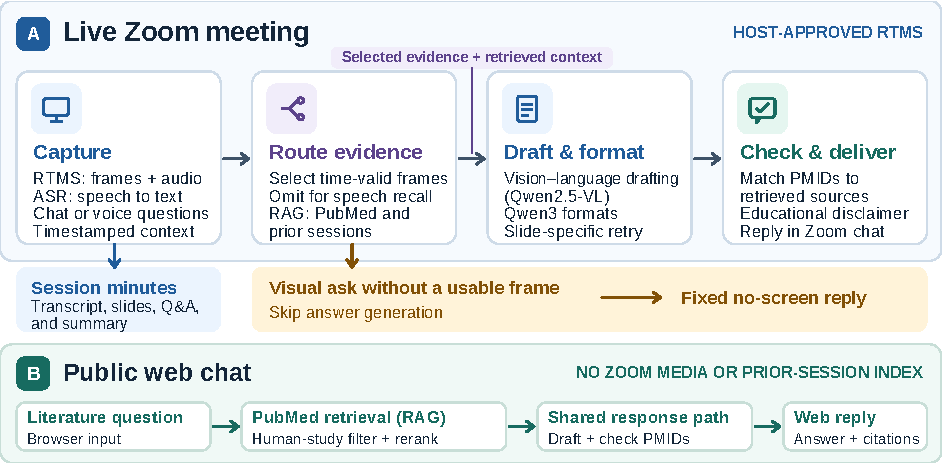
\includegraphics[width=\textwidth]{architecture_refined.pdf}

\caption{ECHO-AI architecture. RTMS = Real-Time Media Streams; VL = vision--language; ASR = automatic speech recognition; RAG = retrieval-augmented generation. The public web interface has no access to live meeting media or prior-session indexes. Visual questions without frames bypass generation and return a fixed reply.}\label{fig:architecture}\end{figure*}

\subsection{Live Meeting Context}

With host approval, ECHO-AI joins a Zoom meeting and receives shared-screen images and audio via RTMS. Participants interact through public mentions, private chat, or voice. Faster-Whisper runs Whisper large-v3 for automatic speech recognition (ASR) (Radford et al., 2023).\footnote{\href{https://github.com/SYSTRAN/faster-whisper}{Faster-Whisper implementation} and \href{https://huggingface.co/openai/whisper-large-v3}{Whisper large-v3 model card}.} Frame deduplication retains distinct visual context. Frames are selected at or before the question timestamp, preserving the temporal relationship between a question and the displayed material.

\subsection{Question Routing and Evidence Retrieval}

\textbf{Select meeting context.} Rules classify each question as visual, speech-related, or general. General questions use the available textual context. A question about the current slide calls for screen images. A question about what a participant said calls for the transcript, so the assistant leaves out the images.

\textbf{Retrieve supporting material.} A separate decision determines whether to retrieve material from PubMed, the prior-session index, or both. Questions that require no retrieval proceed with the selected meeting context. ECHO-AI retrieves PubMed articles, filters for human studies, and reranks the abstracts (Sayers et al., 2022). It also expands ambiguous medical abbreviations. The prior-session index contains \textbf{3,310 overlapping transcript chunks} from \textbf{98 ECHO session recordings}. Lexical search matches query terms, while semantic embeddings help find related passages. ECHO-AI combines these methods to search the de-identified transcripts (Robertson and Zaragoza, 2009; Chen et al., 2024).

\subsection{Answer Generation and Delivery}

A visual question first passes through an availability check. If no usable frame is available, ECHO-AI returns a fixed screen-unavailable reply and skips answer generation. We call this response abstention. For questions that proceed to generation, Qwen2.5-VL (Bai et al., 2025) drafts from the selected context. For slide questions, a retry asks the model to describe the slide if the first draft repeats page labels.

Qwen3 (Yang et al., 2025), a large language model (LLM), formats the answer. Before displaying the references, ECHO-AI checks each PubMed identifier (PMID) against the list returned by retrieval. Clinical replies carry an educational-use disclaimer.

A wake phrase activates voice questions. After a successful answer, a cooldown briefly delays further replies. When a session ends, the minutes module saves a transcript, sampled slides, the questions and answers, and a summary. Appendix~B lists hardware and replay commands.

\subsection{Implementation, Licensing, and Public Access}

Node.js orchestrates the bot; Python/vLLM hosts models on local GPUs. \textbf{License:} sanitized meeting-bot and website source are \textbf{MIT}; model weights keep upstream licenses (Qwen2.5-VL-3B-Instruct is non-commercial research; Qwen3-4B-Instruct-2507 is Apache-2.0; BGE-M3 is MIT). The release excludes credentials, private media, and institutional transcript indexes. The live meeting path requires institutional Zoom infrastructure. The public demo provides PubMed lookup through the configured GPU model services.

\textbf{Reviewer codebase.} The \href{https://github.com/238Plutonium/echo-ai-naacl-submission/tree/fef2ac3d2a907faeeb7c71ac52b4e60260be3060}{released source} has three entry points. \nolinkurl{meeting-bot/} contains the Zoom bot, \nolinkurl{website/} contains the public interface, and \nolinkurl{evaluation/} contains the fixtures, saved outputs, and validation scripts. The recorded replay viewer runs on a CPU. Generating new answers requires the model services described in Appendix~B.

\needspace{6\baselineskip}
\section{System Demonstration}\label{sec:demo}

\textbf{Ask about the slide.} During an opioid use disorder discussion, a facilitator asks ECHO-AI to explain the slide on screen (Figure~\ref{fig:demo}a). The assistant selects a frame from the time of the question and uses it to answer.

\textbf{Ask what was said.} A follow-up about a speaker's comment uses the transcript. In the synthetic timing replay, the slide shows \texttt{13:30} and the facilitator says \texttt{08:30}. A question about the spoken time calls for \texttt{08:30}, while a question about the slide calls for \texttt{13:30}.

\begin{figure*}[t]\centering
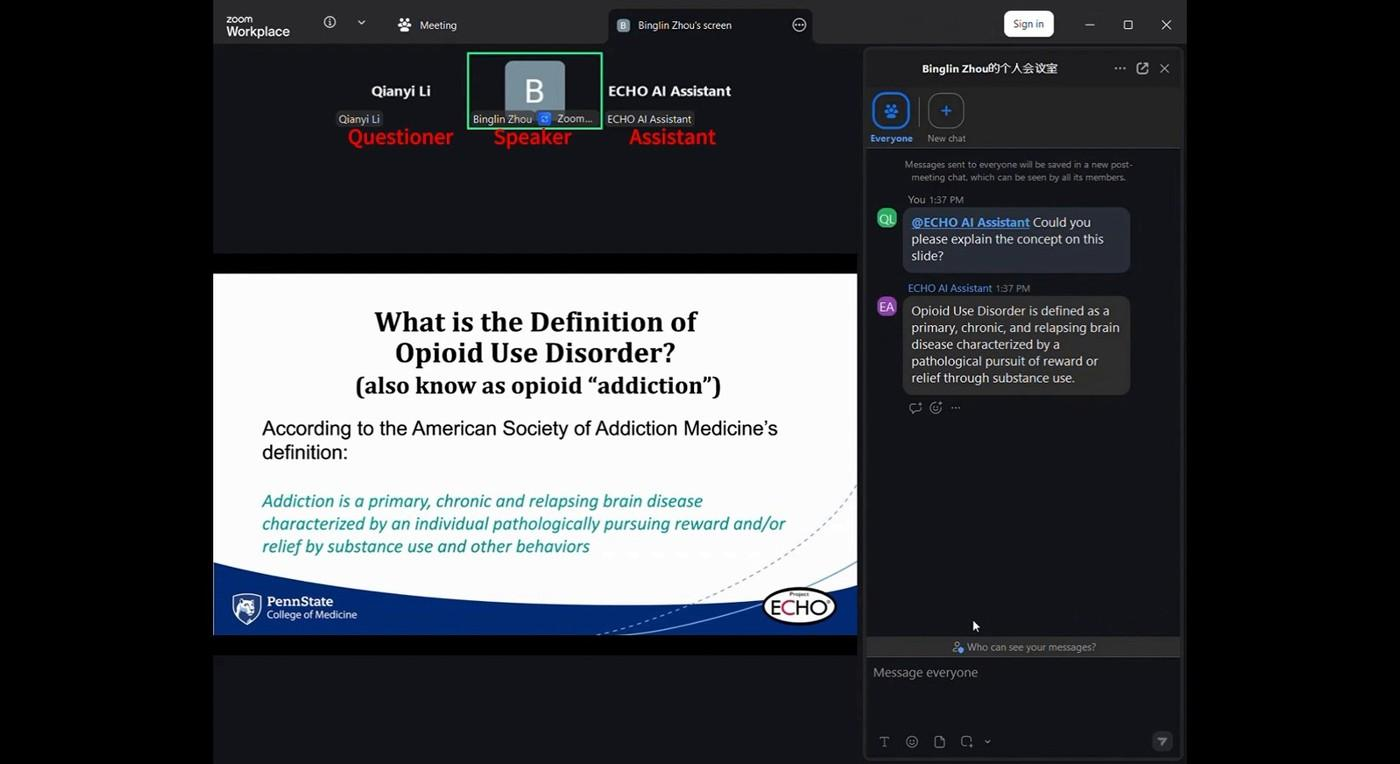
\includegraphics[width=.485\textwidth]{image5.jpeg}\hfill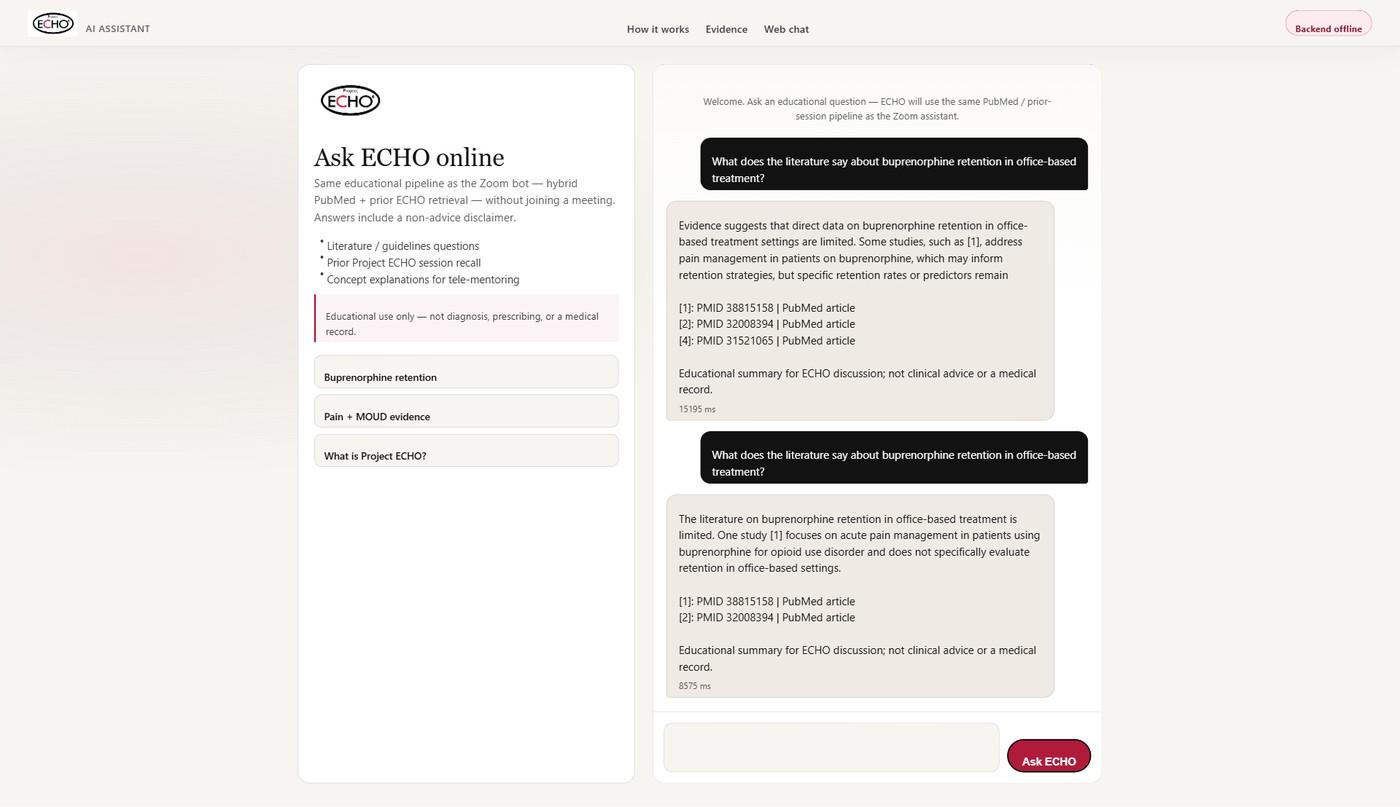
\includegraphics[width=.485\textwidth]{image6.jpeg}

\caption{(a) ECHO-AI answering a slide question within Zoom (left); (b) the public literature interface displaying responses with PubMed identifiers (right).}\label{fig:demo}\end{figure*}

\begin{table*}[t]\centering\small\setlength{\tabcolsep}{3pt}

\begin{tabularx}{\textwidth}{@{}p{.18\textwidth}p{.12\textwidth}p{.20\textwidth}p{.20\textwidth}X@{}}\toprule

\textbf{System} & \textbf{Live meeting} & \textbf{Screen and ASR} & \textbf{Medical RAG} & \textbf{Q\&A interface}\\\midrule

MedTutor & --- & --- & Textbooks + PubMed and Semantic Scholar & Web UI\\

Zoom AI Companion & Yes & ASR; optional screen OCR & --- & Meeting Q\&A\\

Otter AI Chat & Yes & ASR; captured slides & --- & Transcript and slide Q\&A\\

Fireflies AskFred & Google Meet via extension & ASR & --- & Transcript chat\\

ECHO-AI & Zoom bot & Deskshare + ASR & PubMed + prior ECHO & Chat + voice\\

\bottomrule\end{tabularx}

\caption{Documented features as of November 2026. A dash indicates that the sources reviewed do not document a dedicated feature in that category. Tables~\ref{tab:routing} and~\ref{tab:classifiers} report the controlled comparisons.}\end{table*}

\textbf{Look up a source.} A request for a PubMed source returns an answer with checked PubMed identifiers. A question about earlier teaching can search the prior-session index. After the call, the facilitator can review the transcript, sampled slides, questions and answers, and summary.

\textbf{Try the workflow.} Open the public PubMed chat (Figure~\ref{fig:demo}b) and try ``What is buprenorphine used for in opioid use disorder?'' When retrieval succeeds, the interface presents an educational summary with numbered PMID citations. Readers can follow those identifiers to the source abstracts.

For the meeting path, watch the narrated screencast to see the Zoom interaction. Then open \nolinkurl{evaluation/recorded_replay/index.html} and select VIS-ZERO-01. The viewer pairs the replies for a single visual question and shows the attached-frame count and guard setting. Appendix~A gives worked examples, and Appendix~B explains how to run the installable replay.

\section{System Evaluation}\label{sec:eval}

We evaluate evidence selection, answer quality, and the experience of using ECHO-AI. The upstream tests examine which context reaches the answer models. The downstream tests assess the resulting replies and their citations. A staff survey assesses the interaction during a case-based demonstration.

\subsection{Upstream Evaluation: Evidence Selection}\label{sec:upstream}

\textbf{Meeting log.} We analyzed 419 answers (289 distinct answer strings) to project-team questions across 55 Zoom streams. Of 122 slide questions, 86 had an attached frame (70.5\%). Frame fingerprinting compares image signatures to remove repeated screen content. It kept 290 images and removed 19,078 near-duplicates. Across all answers, 227 had no frames, 129 had one, 20 had two, and 43 had three.

Of the 52 answers with a retrieval record, 33 used PubMed, 14 used PubMed and prior sessions, and five used prior sessions alone. The log covers the meeting workflow. Table~\ref{tab:deployment} summarizes the measurements. The log shows the assistant using visual context and both retrieval sources within the meeting workflow.

\textbf{Response time.} The log includes end-to-end timing for 213 of the 419 answers. The average was 6.0 seconds and the median was 4.1 seconds. In a separate sample of 58 interactions, the time from voice activation to question submission averaged 7.8 seconds. These timings suggest that answers can arrive while the case discussion is still in progress.

\begin{table}[t]\centering\small\setlength{\tabcolsep}{3pt}

\begin{tabularx}{\columnwidth}{@{}>{\raggedright\arraybackslash}p{.37\columnwidth}>{\raggedright\arraybackslash}X@{}}\toprule

\textbf{Metric} & \textbf{Measured value}\\\midrule

Logged answers & 419; 289 distinct answer strings\\

Frame attachment & 86/122 slide questions (70.5\%)\\

PMID provenance & 27/27 PMID-bearing answers used IDs in retrieved evidence\\

Full-pipeline latency & Mean 6.0 s; median 4.1 s (n = 213)\\

Facilitator usability & 4.13/5; 15 items (53 scored, 7 unable)\\

Human answer packet & 4.26/5 equal-rater mean (3 raters, 13 items)\\

\bottomrule\end{tabularx}

\caption{Deployment and evaluation at a glance. The development log, answer packet, and facilitator survey cover different samples.}\label{tab:deployment}\end{table}

\textbf{Choosing the source.} We tested two routing decisions (Table~\ref{tab:classifiers}). The focus test asks whether the question refers to speech, a slide, or neither (30, 38, and 10 questions). The retrieval test asks which source is needed (eight literature, four prior-session, and 20 no-retrieval questions). Reference labels came from the experiment categories and synthetic probes. Accuracy is the fraction of predictions that match those labels. Qwen3-4B serves as an LLM classifier. Each always-select baseline assigns the same label to every question.

\begin{table}[t]\centering\small\setlength{\tabcolsep}{4pt}
\begin{tabularx}{\columnwidth}{@{}>{\raggedright\arraybackslash}Xr@{}}\toprule
\textbf{Setting} & \textbf{Result}\\\midrule
\multicolumn{2}{@{}l@{}}{\textit{Speech recall with a conflicting slide}}\\
\multicolumn{2}{@{}l@{}}{\textit{Replies mentioning the spoken value}}\\
Use transcript, withhold slide & 90/90 (100\%)\\
Use transcript and slide & 56/90 (62.2\%)\\\midrule
\multicolumn{2}{@{}l@{}}{\textit{Visual questions with no screen image}}\\
\multicolumn{2}{@{}l@{}}{\textit{Replies that abstain from describing the screen}}\\
Availability check enabled & 33/35 (94.3\%)\\
Availability check disabled & 3/35 (8.6\%)\\
\bottomrule\end{tabularx}
\caption{Two paired replay tests. Speech recall uses 30 cases repeated three times per setting. The visual test uses 35 questions per setting. Abstention means reporting that screen content is unavailable.}\label{tab:routing}
\end{table}

\begin{table}[t]\centering\small\setlength{\tabcolsep}{4pt}
\begin{tabularx}{\columnwidth}{@{}>{\raggedright\arraybackslash}Xrr@{}}\toprule
\textbf{Method} & \textbf{Correct} & \textbf{Time (ms)}\\\midrule
\multicolumn{3}{@{}l@{}}{\textit{Choose speech, slide, or general context (78 questions)}}\\
ECHO-AI rules & 73/78 & 0.028\\
Qwen3-4B classifier & 75/78 & 49.8\\
Always choose slide & 38/78 & ---\\\midrule
\multicolumn{3}{@{}l@{}}{\textit{Choose retrieval source or none (32 questions)}}\\
ECHO-AI rules & 22/32 & 0.221\\
Qwen3-4B classifier & 15/32 & 68.7\\
Always skip retrieval & 20/32 & ---\\
\bottomrule\end{tabularx}
\caption{Routing accuracy and speed. Correct is the number of predictions matching the category-derived labels. Time is the mean per routing decision in milliseconds. Lower times mean faster routing. Dashes indicate unreported timing.}\label{tab:classifiers}
\end{table}

For focus, the rules matched 73 of 78 labels and Qwen3-4B matched 75. Across all 32 retrieval questions, the rules matched 22 labels, Qwen3-4B matched 15, and the always-none baseline matched 20. Among the 12 questions that required retrieval, the rules matched six, Qwen3-4B matched 12, and the always-literature baseline matched eight. The rules took less than 1 ms on average for either decision. The focus results support efficient context selection. Across the tested question mix, rule-based retrieval routing also matched more reference labels than the LLM classifier.

\textbf{When the screen frame is missing.} We sent the same 35 synthetic visual questions through the pipeline with no frames attached. Each question was run with the availability check (guard) on and off. Enabling the guard increased abstentions from 3/35 to 33/35. Thirty-one questions triggered abstention only with the guard and one only without it. The net gain was 85.7 percentage points, $(31-1)/35$ (two-sided exact McNemar $p=1.54\times10^{-8}$).

The guard can answer immediately with a screen-unavailable reply. In this replay, mean latency fell from 1{,}524 to 374 ms and the median from 865.3 to 3.2 ms. Appendix~B links to the paired outputs and item-level labels. Together, these results show that checking visual availability helps the assistant communicate when it lacks screen evidence and respond promptly.

\textbf{Recalling a spoken detail.} In 30 synthetic cases, the speaker said one value and the slide displayed another. We asked for the spoken value three times per case in each condition. When the slide was withheld, replies contained the spoken value in 90 of 90 runs, compared with 56 of 90 when the slide was attached. The metrics count mentions of the spoken value and mentions of the slide value alone. Slide-only replies went from 37.8\% to 0\%. The case-mean changes for the spoken and slide-only values were $+0.38$ and $-0.38$, respectively. Appendix~A shows a worked example. The paired comparison supports selecting context according to the question to preserve spoken details when a slide conflicts with speech.

\textbf{Checking retrieved literature.} The literature workflow applies the PubMed Humans[Mesh] filter before reranking the returned abstracts. In a targeted title-query check, the filter excluded the veterinary guideline PMID 29314873 from new retrieval. This check demonstrates the intended filtering behavior for that source. Appendix~C describes the attribution audit used to evaluate the support provided by abstracts after generation.

\subsection{Downstream Evaluation: Answer Quality}\label{sec:downstream}

Three human graders and a Qwen3-4B judge scored the same 13 archived answers about opioid use disorder and related topics. The packet includes four summaries, three literature requests, three slide requests, one prior-session request, and two other questions. The rubric scores factual appropriateness, contextual grounding, evidence usefulness, safety, and usability. We mapped one grader's 1--3 scores linearly onto the 1--5 scale (1 to 1, 2 to 3, and 3 to 5) and gave each human grader equal weight.

\begin{table}[t]\centering\small\setlength{\tabcolsep}{5pt}
\begin{tabular}{@{}lrr@{}}\toprule
\textbf{Dimension (1--5)} & \textbf{Human} & \textbf{Model}\\\midrule
Factual appropriateness & 4.19 & 4.15 \\
Contextual grounding & 5.00 & 3.62 \\
Evidence usefulness & 3.78 & 3.64 \\
Safety and hedging & 4.51 & 5.00 \\
Usability & 4.12 & 4.85 \\
\textbf{Overall} & \textbf{4.26} & \textbf{4.26} \\
\bottomrule\end{tabular}
\caption{Human and Qwen3-4B ratings of the same 13 answers. The model judge shares the deployed formatter's Qwen3 family.}\label{tab:medtutor}
\end{table}

Contextual grounding measures whether the answer uses the relevant slide or speech. Evidence usefulness measures whether the material helps answer the question. Table~\ref{tab:medtutor} reports each dimension, and Appendix~B links to the rubric. The human score suggests usefulness for the sampled teaching tasks.

\textbf{Citation provenance.} Twenty-seven answers cite 44 distinct PMIDs; every ID appears in the retrieval record. Twenty-five of the 27 answers include an educational-use sentence. Appendix~C records the audit examples. This result makes the displayed identifiers traceable to the material returned by retrieval.

\textbf{Claim support.} An ALCE-style audit (Gao et al., 2023; \nolinkurl{evaluation/citation_faithfulness/}) uses a same-family Qwen3-4B judge to score 114 claim--citation pairs from 86 statements in 28 answers against PubMed abstracts. Scores are 0 (unsupported), 0.5 (partial), or 1 (full support). At threshold $\tau$, let $C_\tau$ count pairs scoring at least $\tau$ and $S_\tau$ count statements with at least one such citation.
\[
\mathrm{Precision}(\tau)=\frac{C_\tau}{114},\qquad
\mathrm{Recall}(\tau)=\frac{S_\tau}{86}.
\]
Full support covers 22 pairs and 20 statements. Counting 60 partial scores, the automated judge found support for most claim--citation pairs (82/114) and at least one supporting citation for 63/86 statements (Table~\ref{tab:cite}). PMID provenance measures retrieval membership. The automated attribution audit estimates claim support against abstracts. These scores suggest that retrieved abstracts provided supporting evidence for most audited statements at the partial-or-full threshold.

\begin{table}[t]\centering\small\setlength{\tabcolsep}{4pt}
\begin{tabularx}{\columnwidth}{@{}Xr@{}}\toprule
\textbf{ALCE-style metric} & \textbf{Value}\\\midrule
Citation precision (attr$\geq$0.5) & 0.72\\
Citation recall (attr$\geq$0.5) & 0.73\\
\bottomrule\end{tabularx}
\caption{Automatic citation attribution vs.\ PubMed abstracts (Qwen3-4B judge; same family as the formatter).}\label{tab:cite}
\end{table}

\subsection{Human--Model Agreement}\label{sec:agreement}

Across the five rubric dimensions, the human and model averages both round to 4.26/5 (Table~\ref{tab:medtutor}). At the item level, the pooled human and model ratings were within one point on 12 of 13 answers, with a mean absolute difference of 0.43 points and a Spearman rank correlation of $\rho{\approx}0.34$. These metrics measure score proximity and ranking agreement, respectively. The \href{https://github.com/238Plutonium/openreview/blob/main/evaluation/packet_scores.csv}{released packet scores} contain the item means. The score proximity suggests potential for automated scoring to assist routine answer review.

\textbf{Generator evaluation.} We used the same 13 questions for a separate exploratory evaluation of text-only generators. Appendix~B reports the archived ECHO-AI reference scores, the standalone model results, and how the judge was configured for each run. These reference scores provide a reproducible basis for examining alternative answer models.

\subsection{Facilitator Usability and Educational Usefulness}

Four Project ECHO staff completed a survey after the September 10, 2026 demonstration. Three watched the session and one asked questions in chat. Across 15 usability items, they gave an average score of 4.13/5 (53 scored responses and seven marked unable to judge). Appeal, ease of use, and question clarity each averaged 4.50/5. Staff asked for quieter replies and the option to let only the facilitator invoke the assistant. The release includes both controls. The feedback suggests a promising fit with case-based discussion.

Staff rated educational usefulness 4.00/5 ($n{=}4$) based on their experience during the demonstration. This rating reflects a positive staff impression of the assistant as a teaching aid. The released \href{https://github.com/238Plutonium/openreview/tree/main/evaluation/education_outcomes}{pre/post questionnaire} supports a follow-up study comparing learner responses before and after a session.

We also used ECHO-AI during the October~27, 2026 Penn State ASERT Project ECHO session. The ratings above come from the September demonstration.

\section{Conclusion}

ECHO-AI lets Project ECHO participants ask about a slide, a spoken detail, or a published study during the same Zoom discussion. In the replay tests, selecting the transcript improved recall of spoken details. The availability check helped the assistant tell participants when it could not see the screen.

Reviewers can explore these behaviors through the meeting screencast, public PubMed chat, and offline replay. Staff feedback identifies which parts of the interaction worked well. The answer packet and released rubric provide a basis for independent clinical review and a study of learning outcomes.

\section*{Limitations}

The evaluation covers project-team queries, four staff ratings from one demonstration, three packet graders, and controlled replay cases. The citation and packet judges share the formatter's Qwen3 family. A follow-up study could assess clinical accuracy, slide interpretation, and learning outcomes.

\section*{Acknowledgments}

We thank Rui Zhang for manuscript feedback and Laura Felix, Jennifer Kraschnewski, Ashmita Grewal, Jessica Beiler, Ellie Hogentogler, Caitlin Kline, Melissa Huffman, Sesi Whaley, and Guido Cervone for supporting the demonstration. Cursor was used to proofread source code.

\clearpage
\nobalance
\section*{Ethics Statement}

ECHO-AI is an educational aid for MOUD and related Project ECHO tele-mentoring. It is not intended to diagnose, prescribe, or create medical records. The system appends the following disclaimer to clinical questions or questions with retrieval records: ``Educational summary for ECHO discussion; not clinical advice or a medical record.'' The host controls admission. PubMed queries use sanitized medical concepts and do not forward raw meeting audio or slide images. Meeting audio and institutional indexes remain subject to the project's institutional retention rules; the public interface queries PubMed only.

\textbf{Patient privacy.} Live ECHO sessions may discuss de-identified clinical cases. Prior-session chunks undergo an automatic redaction pass before indexing; automatic redaction is not a manual privacy certification. Index access is limited to the institutional Zoom path.

Facilitator feedback and the September 2026 recording come from a scheduled demonstration with volunteer Project ECHO and Penn State Institute for Computational and Data Sciences participants. The paper reports staff feedback and excludes patient case text and identifiable patient data.


\clearpage
\begin{thebibliography}{31}

\bibitem[Arora et al.(2010)]{ref2}Sanjeev Arora, Summers Kalishman, Karla Thornton, Denise Dion, Glen Murata, Paulina Deming, Brooke Parish, John Brown, Miriam Komaromy, Kathleen Colleran, Arthur Bankhurst, Joanna Katzman, Michelle Harkins, Luis Curet, Ellen Cosgrove, and Wesley Pak. 2010. Expanding access to hepatitis C virus treatment---extension for community healthcare outcomes (ECHO) project: Disruptive innovation in specialty care. Hepatology, 52(3):1124--1133.

\bibitem[Arora et al.(2011a)]{ref3}Sanjeev Arora, Summers Kalishman, Denise Dion, Dara Som, Karla Thornton, Arthur Bankhurst, Jeanne Boyle, Michelle Harkins, Keith Moseley, Glen Murata, Miriam Komaromy, Joanna Katzman, Kathleen Colleran, Paulina Deming, and Sean Yutzy. 2011a. Partnering urban academic medical centers and rural primary care clinicians to provide complex chronic disease care. Health Affairs, 30(6):1176--1184.

\bibitem[Arora et al.(2011b)]{ref4}Sanjeev Arora, Karla Thornton, Glen Murata, Paulina Deming, Summers Kalishman, Denise Dion, Brooke Parish, Thomas Burke, Wesley Pak, Jeffrey Dunkelberg, Martin Kistin, John Brown, Steven Jenkusky, Miriam Komaromy, and Clifford Qualls. 2011b. Outcomes of treatment for hepatitis C virus infection by primary care providers. New England Journal of Medicine, 364(23):2199--2207.

\bibitem[Bai et al.(2025)]{ref5}Shuai Bai, Keqin Chen, Xuejing Liu, Jialin Wang, Wenbin Ge, Sibo Song, Kai Dang, Peng Wang, Shijie Wang, Jun Tang, Humen Zhong, Yuanzhi Zhu, Mingkun Yang, Zhaohai Li, Jianqiang Wan, et al. 2025. Qwen2.5-VL technical report. arXiv preprint arXiv:2502.13923.

\bibitem[Carletta et al.(2006)]{ref6}Jean Carletta, Simone Ashby, Sebastien Bourban, Mike Flynn, Mael Guillemot, Thomas Hain, Jaroslav Kadlec, Vasilis Karaiskos, Wessel Kraaij, Melissa Kronenthal, Guillaume Lathoud, Mike Lincoln, Agnes Lisowska, Iain McCowan, Wilfried Post, Dennis Reidsma, and Pierre Wellner. 2006. The AMI meeting corpus: A pre-announcement. In Machine Learning for Multimodal Interaction (MLMI), Lecture Notes in Computer Science, pages 28--39.

\bibitem[Chen et al.(2024)]{ref7}Jianlyu Chen, Shitao Xiao, Peitian Zhang, Kun Luo, Defu Lian, and Zheng Liu. 2024. M3-Embedding: Multi-linguality, multi-functionality, multi-granularity text embeddings through self-knowledge distillation. In Findings of the Association for Computational Linguistics: ACL 2024, pages 2318--2335, Bangkok, Thailand. Association for Computational Linguistics.

\bibitem[Fireflies.ai(n.d.)]{ref8}Fireflies.ai. n.d. How to use AskFred during live meetings. \url{https://guide.fireflies.ai/articles/4228644685}. Accessed 25 Nov 2026.

\bibitem[Gao et al.(2023)]{ref9}Tianyu Gao, Howard Yen, Jiatong Yu, and Danqi Chen. 2023. Enabling large language models to generate text with citations. In Proceedings of the 2023 Conference on Empirical Methods in Natural Language Processing, pages 6465--6488, Singapore. Association for Computational Linguistics.

\bibitem[Hu et al.(2023)]{ref10}Yebowen Hu, Timothy Ganter, Hanieh Deilamsalehy, Franck Dernoncourt, Hassan Foroosh, and Fei Liu. 2023. MeetingBank: A benchmark dataset for meeting summarization. In Proceedings of the 61st Annual Meeting of the Association for Computational Linguistics (Volume 1: Long Papers), pages 16409--16423, Toronto, Canada. Association for Computational Linguistics.

\bibitem[Hu et al.(2026)]{ref11}Yuelin Hu, Jun Xu, Bingcong Lu, Zhengxue Cheng, Hongwei Hu, Ronghua Wu, and Li Song. 2026. MeetBench-XL: Calibrated multi-dimensional evaluation and learned dual-policy agents for real-time meetings. arXiv preprint arXiv:2602.03285.

\bibitem[Jang et al.(2025)]{ref12}Dongsuk Jang, Ziyao Shangguan, Kyle Tegtmeyer, Anurag Gupta, Jan Czerminski, Sophie Chheang, and Arman Cohan. 2025. MedTutor: A retrieval-augmented LLM system for case-based medical education. In Proceedings of the 2025 Conference on Empirical Methods in Natural Language Processing: System Demonstrations, pages 319--353, Suzhou, China. Association for Computational Linguistics.

\bibitem[Ji et al.(2023)]{ref13}Ziwei Ji, Nayeon Lee, Rita Frieske, Tiezheng Yu, Dan Su, Yan Xu, Etsuko Ishii, Ye Jin Bang, Andrea Madotto, and Pascale Fung. 2023. Survey of hallucination in natural language generation. ACM Computing Surveys, 55(12), article 248, pages 1--38.

\bibitem[Jin et al.(2019)]{ref14}Qiao Jin, Bhuwan Dhingra, Zhengping Liu, William W. Cohen, and Xinghua Lu. 2019. PubMedQA: A dataset for biomedical research question answering. In Proceedings of the 2019 Conference on Empirical Methods in Natural Language Processing and the 9th International Joint Conference on Natural Language Processing (EMNLP-IJCNLP), pages 2567--2577, Hong Kong, China. Association for Computational Linguistics.

\bibitem[Karpukhin et al.(2020)]{ref15}Vladimir Karpukhin, Barlas Oguz, Sewon Min, Patrick Lewis, Ledell Wu, Sergey Edunov, Danqi Chen, and Wen-tau Yih. 2020. Dense passage retrieval for open-domain question answering. In Proceedings of the 2020 Conference on Empirical Methods in Natural Language Processing (EMNLP), pages 6769--6781, Online. Association for Computational Linguistics.

\bibitem[Lewis et al.(2020)]{ref16}Patrick Lewis, Ethan Perez, Aleksandra Piktus, Fabio Petroni, Vladimir Karpukhin, Naman Goyal, Heinrich Küttler, Mike Lewis, Wen-tau Yih, Tim Rocktäschel, Sebastian Riedel, and Douwe Kiela. 2020. Retrieval-augmented generation for knowledge-intensive NLP tasks. In Advances in Neural Information Processing Systems, volume 33, pages 9459--9474.

\bibitem[Manakul et al.(2023)]{ref17}Potsawee Manakul, Adian Liusie, and Mark Gales. 2023. SelfCheckGPT: Zero-resource black-box hallucination detection for generative large language models. In Proceedings of the 2023 Conference on Empirical Methods in Natural Language Processing, pages 9004--9017, Singapore. Association for Computational Linguistics.

\bibitem[Otter.ai(n.d.)]{ref19}Otter.ai. n.d. Automated slide capture overview. \url{https://help.otter.ai/hc/en-us/articles/5093321813911}. Accessed 25 Nov 2026.

\bibitem[Yang et al.(2025)]{ref20}An Yang et al. 2025. Qwen3 technical report. arXiv preprint arXiv:2505.09388.

\bibitem[Radford et al.(2023)]{ref21}Alec Radford, Jong Wook Kim, Tao Xu, Greg Brockman, Christine McLeavey, and Ilya Sutskever. 2023. Robust speech recognition via large-scale weak supervision. In Proceedings of the 40th International Conference on Machine Learning, volume 202 of Proceedings of Machine Learning Research, pages 28492--28518. PMLR.

\bibitem[Robertson and Zaragoza(2009)]{ref22}Stephen E. Robertson and Hugo Zaragoza. 2009. The probabilistic relevance framework: BM25 and beyond. Foundations and Trends in Information Retrieval, 3:333--389.

\bibitem[Sayers et al.(2022)]{ref23}Eric W. Sayers, Evan E. Bolton, J. Rodney Brister, Kathi Canese, Jessica Chan, Donald C. Comeau, Ryan Connor, Kathryn Funk, et al. 2022. Database resources of the national center for biotechnology information. Nucleic Acids Research, 50(D1):D20--D26.

\bibitem[Tu et al.(2025)]{ref26}Tao Tu, Mike Schaekermann, Anil Palepu, Khaled Saab, Jan Freyberg, Ryutaro Tanno, Amy Wang, Brenna Li, Mohamed Amin, Yong Cheng, Elahe Vedadi, Nenad Tomasev, Shekoofeh Azizi, Karan Singhal, et al. 2025. Towards conversational diagnostic artificial intelligence. Nature, 642(8067):442--450.

\bibitem[Xiong et al.(2024)]{ref27}Guangzhi Xiong, Qiao Jin, Zhiyong Lu, and Aidong Zhang. 2024. Benchmarking retrieval-augmented generation for medicine. In Findings of the Association for Computational Linguistics: ACL 2024, pages 6233--6251, Bangkok, Thailand. Association for Computational Linguistics.

\bibitem[Zakka et al.(2024)]{ref28}Cyril Zakka, Rohan Shad, Akash Chaurasia, Alex R. Dalal, Jennifer L. Kim, Michael Moor, Robyn Fong, Curran Phillips, Kevin Alexander, Euan Ashley, Jack Boyd, Kathleen Boyd, Karen Hirsch, Curtis Langlotz, Rita Lee, et al. 2024. Almanac---retrieval-augmented language models for clinical medicine. NEJM AI, 1(2).

\bibitem[Zhong et al.(2021)]{ref29}Ming Zhong, Da Yin, Tao Yu, Ahmad Zaidi, Mutethia Mutuma, Rahul Jha, Ahmed Hassan Awadallah, Asli Celikyilmaz, Yang Liu, Xipeng Qiu, and Dragomir Radev. 2021. QMSum: A new benchmark for query-based multi-domain meeting summarization. In Proceedings of the 2021 Conference of the North American Chapter of the Association for Computational Linguistics: Human Language Technologies, pages 5905--5921, Online. Association for Computational Linguistics.

\bibitem[Zoom Video Communications(n.d.-a)]{ref30}Zoom Video Communications. n.d.-a. Realtime Media Streams developer documentation. \url{https://developers.zoom.us/docs/rtms/}. Accessed 25 Nov 2026.

\bibitem[Zoom Video Communications(n.d.-b)]{ref31}Zoom Video Communications. n.d.-b. Asking in-meeting questions with AI. \url{https://support.zoom.com/hc/en/article?id=zm_kb&sysparm_article=KB0057748}. Accessed 25 Nov 2026.

\end{thebibliography}

\clearpage

\appendix

\balance

\section{Worked Examples and Routing}

\textbf{Literature ask (archived held-out).}
\begin{quote}\small
\emph{Q:} How do you treat dementia patients, citing medpub?\\
\emph{A (body, excerpt):} \ldots Cognitive stimulation therapy (CST) has been associated with improved cognitive function and quality of life in individuals with mild to moderate dementia [3]. \ldots Educational summary for ECHO discussion; not clinical advice or a medical record.\\
\emph{Bibliography (excerpt):} \texttt{[3]: PMID 30336989 | \ldots}
\end{quote}
The footnote resolves to a PMID in the retrieval record. The audit assigned full support to the displayed claim--citation pair (Appendix~C).

\textbf{Speech vs.\ slide conflict (SPEECH-18).} The transcript says \texttt{08:30}, and the slide shows \texttt{13:30}. The replay question asks for the start time the facilitator said to use. With the frame withheld, the transcript time appears in all three replies. With the frame included, all three replies give the slide time and attribute it to the facilitator. This example can be located by case ID in the released speech-recall JSONL alongside its frame count, arm, and repetition number.

\textbf{Zero-frame contrast (VIS-ZERO-01).} The question asks what is on screen right now. The run records no attached frames in either condition. The guard-on answer says no screen-share image is arriving and asks the participant to check screen sharing. With the guard disabled, the answer describes an application workspace despite the missing frame. Both output records and their labels are available in the public replay viewer.

\textbf{Focus rules (sketch).} Slide/``on screen'' $\rightarrow$ attach up to 3 timestamped frames. ``What did \ldots say'' / speech recall $\rightarrow$ withhold frames. Treatment/PubMed/guideline lexemes $\rightarrow$ literature RAG (Humans[Mesh], abstract rerank, top 5). ``Last session''/prior ECHO $\rightarrow$ BM25+embedding over de-identified chunks. Availability gate runs before VL draft.

\textbf{Routing baselines (Table~\ref{tab:classifiers}).} Full prediction tables and category-derived gold files are in \nolinkurl{evaluation/routing_comparison/} (\texttt{python3 run\_routing\_baselines.py}; \texttt{-{}-skip-llm} for CPU-only).

\section{Open-Source Release, Demo Access, and Reproducibility}

\textbf{Release (MIT code).} Repository: \url{https://github.com/238Plutonium/echo-ai-naacl-submission}. Contains sanitized \texttt{meeting-bot/}, PubMed website, \texttt{demo\_replay/} fixtures, \texttt{evaluation/} (recorded no-frame walkthrough, speech-recall ablation, citation faithfulness, claim audit, rubrics), and \texttt{python evaluation/verify\_results.py} offline checks. Excludes Zoom credentials and institutional prior-session indexes.

\textbf{Live demo / video.} PubMed chat: \url{https://chive-shrouded-gag.ngrok-free.dev/chat.html}. Screencast (2:09): \url{https://www.youtube.com/watch?v=WwFCYDoYzm8}. Full Sept.\ 2026 recording: \url{https://psu.mediaspace.kaltura.com/media/t/1_0syzr0gf}.

\textbf{Hardware.} Local GPUs: Whisper large-v3, BGE-M3, Qwen2.5-VL-3B-Instruct, Qwen3-4B-Instruct-2507. Node.js 22+ bot; HTTPS tunnel for RTMS. Key settings: uniqueness cutoff 0.012; \texttt{PRIVATE\_RAG\_BM25\_K=100}, \texttt{PRIVATE\_RAG\_EMBEDDING\_K=3}; up to five reranked PubMed abstracts; up to three frames at/before ask time.

\textbf{Replay without Zoom.} From the repository root, run \nolinkurl{python3 evaluation/verify_results.py} to check published counts. For new answers, follow \nolinkurl{meeting-bot/quick_start.md}, set \texttt{DEMO\_REPLAY\_ENABLED=true} in the bot, and run \texttt{npm run demo:replay} from \texttt{meeting-bot/}. The driver resets a synthetic stream, injects a fixture image and transcript turns, then submits the question to the ask pipeline. The recorded viewer in \nolinkurl{evaluation/recorded_replay/} works without model services.

\textbf{Human packet rubric (1--5).} Factual appropriateness; contextual grounding; evidence usefulness; safety/hedging; usability. Facilitator form: 15 usability items (appeal, ease, non-disruption, voice-wake, \ldots). Sheets and \nolinkurl{evaluation/RUBRIC.md} are in the release; filled individual facilitator sheets stay private. Generator scores: \nolinkurl{evaluation/frontier\_baselines/}. Education-outcome instrument: \nolinkurl{evaluation/education\_outcomes/}.

\newpage\textbf{Inspecting individual cases.} Open \nolinkurl{evaluation/recorded_replay/index.html} for the paired zero-frame outputs and labels. The two runs share the case ID and question and differ in the guard setting. The underlying JSONL records output text, attached-frame count, and latency. For speech conflicts, inspect the included and withheld arms in \nolinkurl{evaluation/speech_recall_ablation/}; group the three repetitions by case before comparing token-mention rates. Replaying the inputs and verifying the archived outputs are separate checks: the former executes current models, while the latter checks the artifact underlying Table~\ref{tab:routing}.

\textbf{Rating materials.} The released packet rubric describes the five scored dimensions and the available labels. The facilitator survey summary reports item means and valid response counts. The three human packet grader means were 5.00, 4.87, and 2.92; their equal-weight average rounds to 4.26/5.

\textbf{Generator comparison.} Table~\ref{tab:generators} contains automated scores for 13 questions per row. Each score averages the five rubric dimensions across those answers. Standalone models received the question text without meeting context or retrieved evidence. Archived answers came from the deployed ECHO-AI workflow. All scores use a Qwen2.5-1.5B-Instruct judge. GGUF is a format for running quantized model weights locally. The Llama-3.2 run used Q4\_K\_M GGUF builds of both generator and judge and changed how the scoring instructions were passed to the judge. The judge saw the question and up to 1,800 characters of each answer. The \href{https://github.com/238Plutonium/openreview/tree/85f3e5969a01605c961e7bc2deb1be49f99965f9/evaluation/frontier_baselines}{evaluation artifacts} include saved generations and item-level scores.

\begin{table}[!ht]\centering\small\setlength{\tabcolsep}{4pt}
\begin{tabularx}{\columnwidth}{@{}Xr@{}}\toprule
\textbf{Generator} & \textbf{Score (/5)}\\\midrule
ECHO-AI (archived) & 3.49\\
Qwen2.5-1.5B-Instruct & 3.82\\
SmolLM2-1.7B-Instruct & 4.12\\
Gemma-2-2B-IT (Q4 GGUF) & 3.72\\
Gemini-3.1-Flash-Lite & 4.86\\
Llama-3.2-3B-Instruct (Q4 GGUF) & 4.31\\
\bottomrule\end{tabularx}
\caption{Exploratory automated scores on the 13-question packet. The last row uses a separate judge configuration.}\label{tab:generators}
\end{table}

\section{Citation Attribution Protocol and Examples}

\textbf{Protocol.} Judge each body assertion--PMID pair against the cited abstract, excluding bibliography lines. Precision averages over pairs and recall counts statements with at least one citation meeting the threshold. At full support (attr$=1$), precision is 0.19 (22/114) and recall is 0.23 (20/86). The table abbreviation attr denotes the judge's attribution score. In this audit, partial support means the abstract supports some of the claim, and full support means it supports the complete claim. Each claim--citation pair is scored separately, so a statement with multiple citations contributes multiple pairs. The Qwen3-4B-Instruct-2507 judge runs at temperature~0. The \nolinkurl{evaluation/citation_faithfulness/} package provides the scores and documented examples.

\textbf{Full support (1).} ``CST has been associated with improved cognitive function \ldots'' $\rightarrow$ \mbox{PMID 30336989}.

\textbf{Partial$=$0.5.} Sleep-hygiene claim $\rightarrow$ PMID 33683929 (human insomnia review). 60/114 instances score 0.5. Table~\ref{tab:cite} includes these scores at attr$\geq$0.5.

\textbf{Lexical screen.} A separate lexical screen finds support for 14/132 pairs (\nolinkurl{evaluation/claim_level_audit/}).

\end{document}
